\documentclass{article}

% If you're new to LaTeX, here's some short tutorials:
% https://www.overleaf.com/learn/latex/Learn_LaTeX_in_30_minutes
% https://en.wikibooks.org/wiki/LaTeX/Basics

% Formatting
\usepackage[utf8]{inputenc}
\usepackage[margin=1in]{geometry}
\usepackage[titletoc,title]{appendix}
\usepackage{wrapfig}
\usepackage[rightcaption]{sidecap}

% Math
% https://www.overleaf.com/learn/latex/Mathematical_expressions
% https://en.wikibooks.org/wiki/LaTeX/Mathematics
\usepackage{amsmath,amsfonts,amssymb,mathtools}

% Images
% https://www.overleaf.com/learn/latex/Inserting_Images
% https://en.wikibooks.org/wiki/LaTeX/Floats,_Figures_and_Captions
\usepackage{graphicx,float}

% Tables
% https://www.overleaf.com/learn/latex/Tables
% https://en.wikibooks.org/wiki/LaTeX/Tables
\usepackage{booktabs}

% Algorithms
% https://www.overleaf.com/learn/latex/algorithms
% https://en.wikibooks.org/wiki/LaTeX/Algorithms
\usepackage[ruled,vlined]{algorithm2e}
\usepackage{algorithmic}

% Code syntax highlighting
% https://www.overleaf.com/learn/latex/Code_Highlighting_with_minted
\usepackage{minted}
\setminted{fontsize=\footnotesize}

% References
% https://www.overleaf.com/learn/latex/Bibliography_management_in_LaTeX
% https://en.wikibooks.org/wiki/LaTeX/Bibliography_Management
\usepackage{biblatex}
\addbibresource{references.bib}

% Title content
\title{Computational Cognitive Science Coursework 2}
\author{s1623705}
\date{March 24, 2020}

\begin{document}

\maketitle

\section{Part 1: Drift Diffusion Process (23 points)}

\subsection{Task (a): Initial Simulations (9)}

The Wiener diffusion process produces the following paths, using the provided parameters and a seed of 0 (which is used in later experiments too):

\begin{figure}[H]
    \centering
    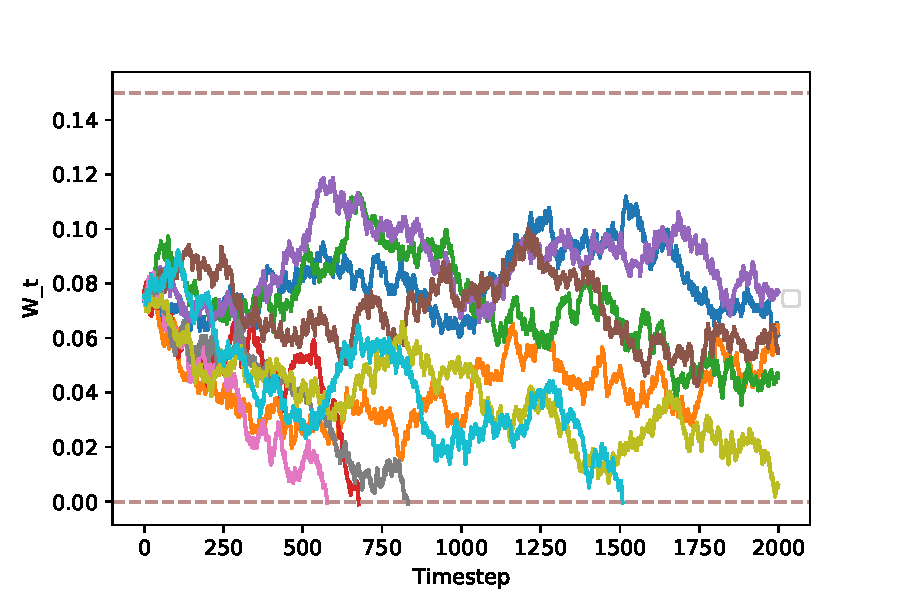
\includegraphics[width=0.8\textwidth]{figures/part1/task1/example_paths.pdf}
    \caption{10 paths produced by the Wiener diffusion process}
    \label{fig:examplepaths}
\end{figure}

The following histograms capture the distribution of response times. To build a better picture of this distribution, 1000 trials have been run:

\begin{figure}[H]
  \centering
  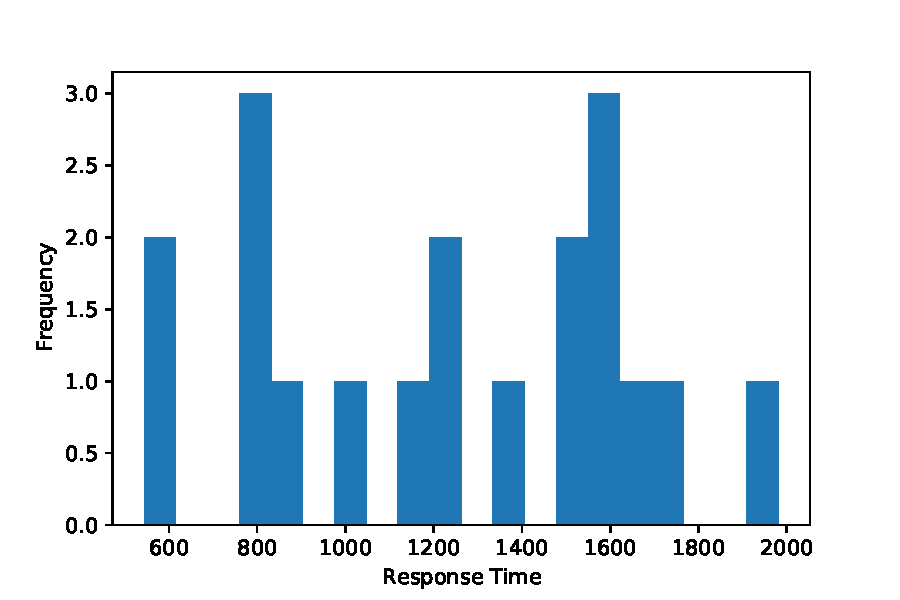
\includegraphics[width=0.4\textwidth]{figures/part1/task1/positive_response_time_histogram.pdf}
  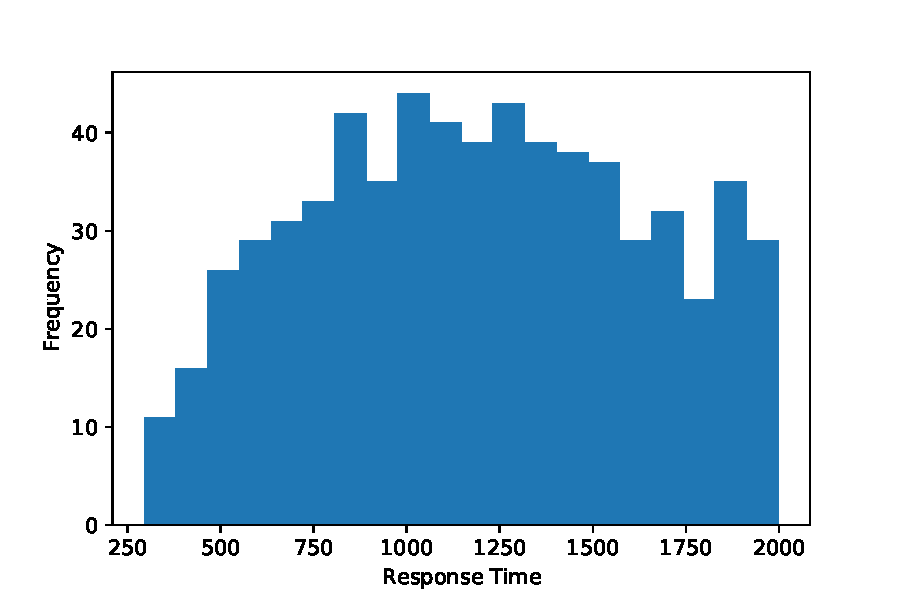
\includegraphics[width=0.4\textwidth]{figures/part1/task1/negative_response_time_histogram.pdf}
  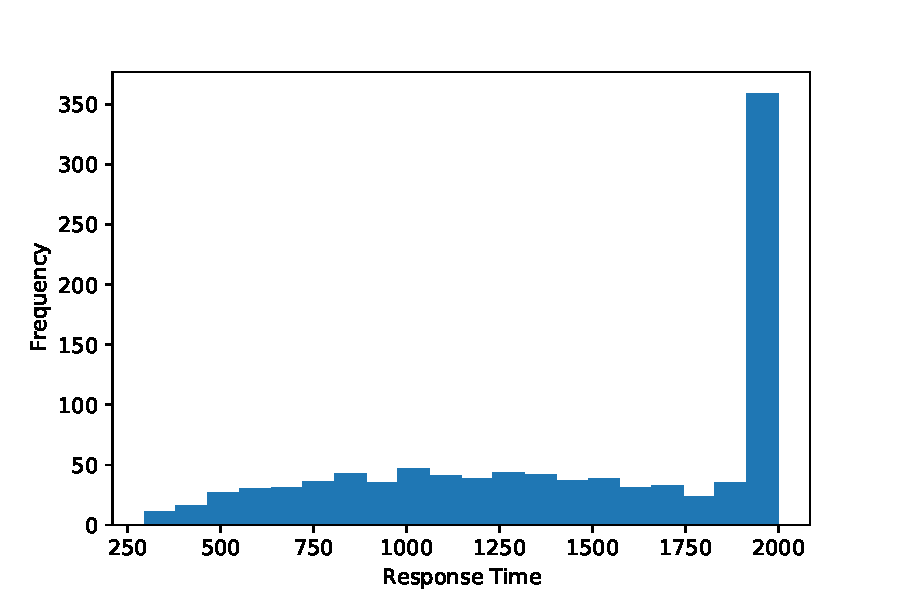
\includegraphics[width=0.4\textwidth]{figures/part1/task1/overall_response_time_histogram.pdf}
  \caption{Positive (left), negative (right) and overall (bottom) response time histograms (1000 trials)}
  \label{fig:responsetimehistograms}
\end{figure}

\begin{table}[h]
  \begin{tabular}{|l|l|l|}
  \hline
  \textbf{Correct}            & \textbf{Incorrect}          & \textbf{Timeout}            \\ \hline
  \multicolumn{1}{|c|}{1.9\%} & \multicolumn{1}{c|}{65.2\%} & \multicolumn{1}{c|}{32.9\%} \\ \hline
  \end{tabular}
  \centering
  \caption{Response constitution (1000 trials)}
  \label{table:responseconstitution}
\end{table}

CAN SOMETHING BE INFERRED ABOUT THE EXPERIMENT?

\subsection{Task (b): Exploring parameter settings (5)}

For a fixed boundary separation of 0.15, drift rates close to 0 cause the accuracy to become close to 0.5, suggesting each new piece of evidence is uninformative. As the drift rate grows positively large, the accuracy tends to 1, whilst growing negatively large tends towards 0. The average response time also grows large as drift rate tends to 0. These results suggest that when the drift rate is informative, a hypothesis is reached both more often and more quickly.

For a fixed mean drift rate of -0.04, small boundary separations allows for a high accuracy, with a low average response time. As boundary separation grows, the accuracy tends to 0, whilst the average response time grows large. This suggests that if the threshold to accept a hypothesis is low, it will be accepted more often, and in a short amount of time.

There is also self-evident dependence between mean drift rate and boundary separation. If the starting position is always inbetween the two hypothesis boundaries, varying the size of mean drift rate and boundary separation together will not have an effect on the accuracy or average response time, as each drift will remain the same relative to the distance of the boundary from the starting point.

\begin{figure}[H]
  \centering
  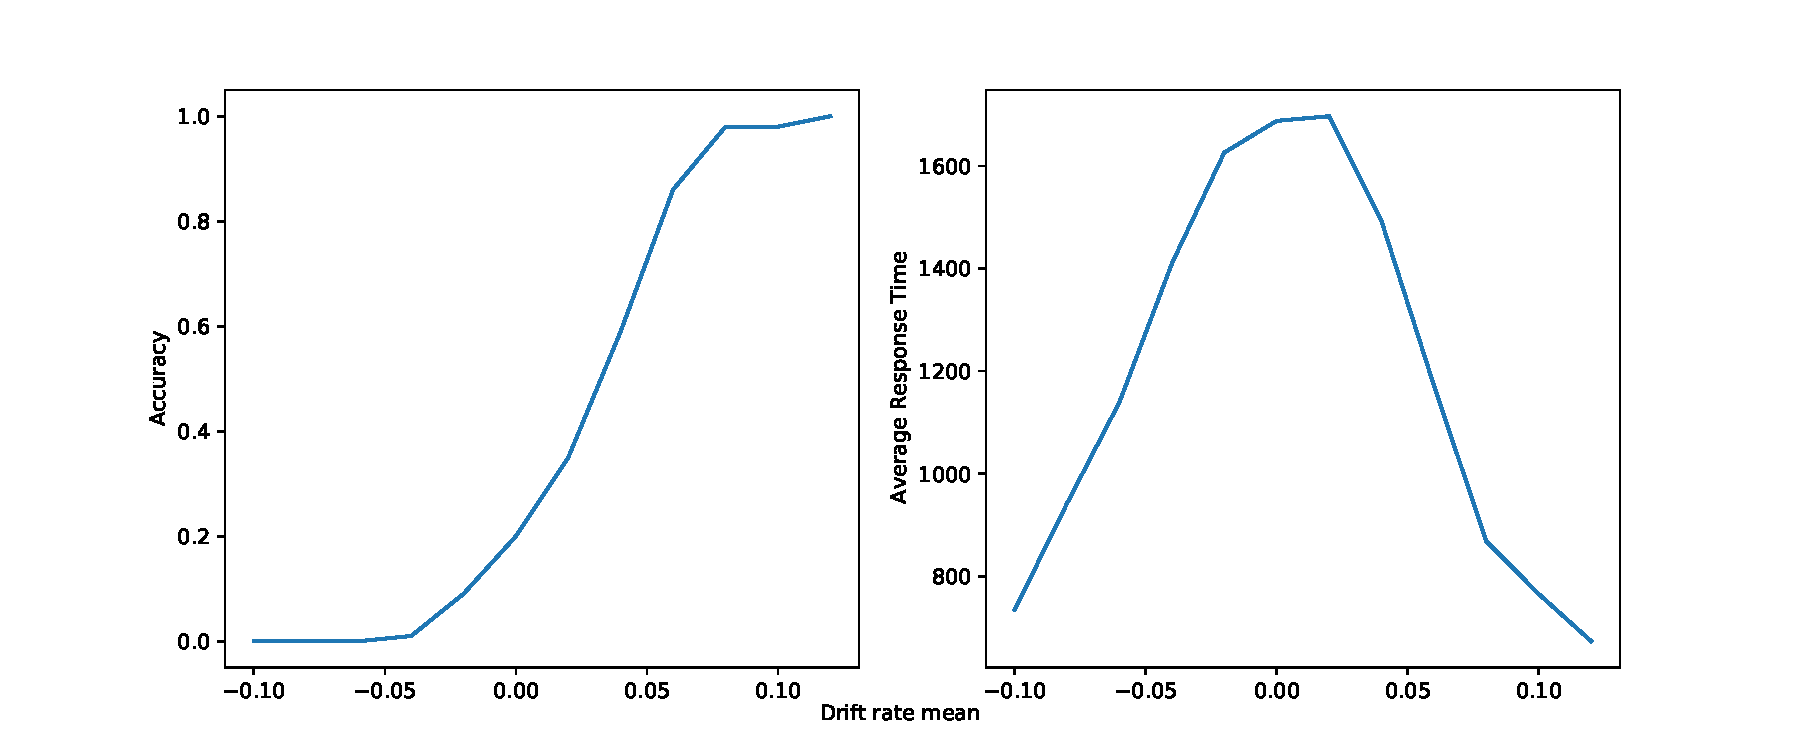
\includegraphics[width=0.8\textwidth]{figures/part1/task2/varying_drift_rate_mean.pdf}
  \label{fig:varyingdriftratemean}
  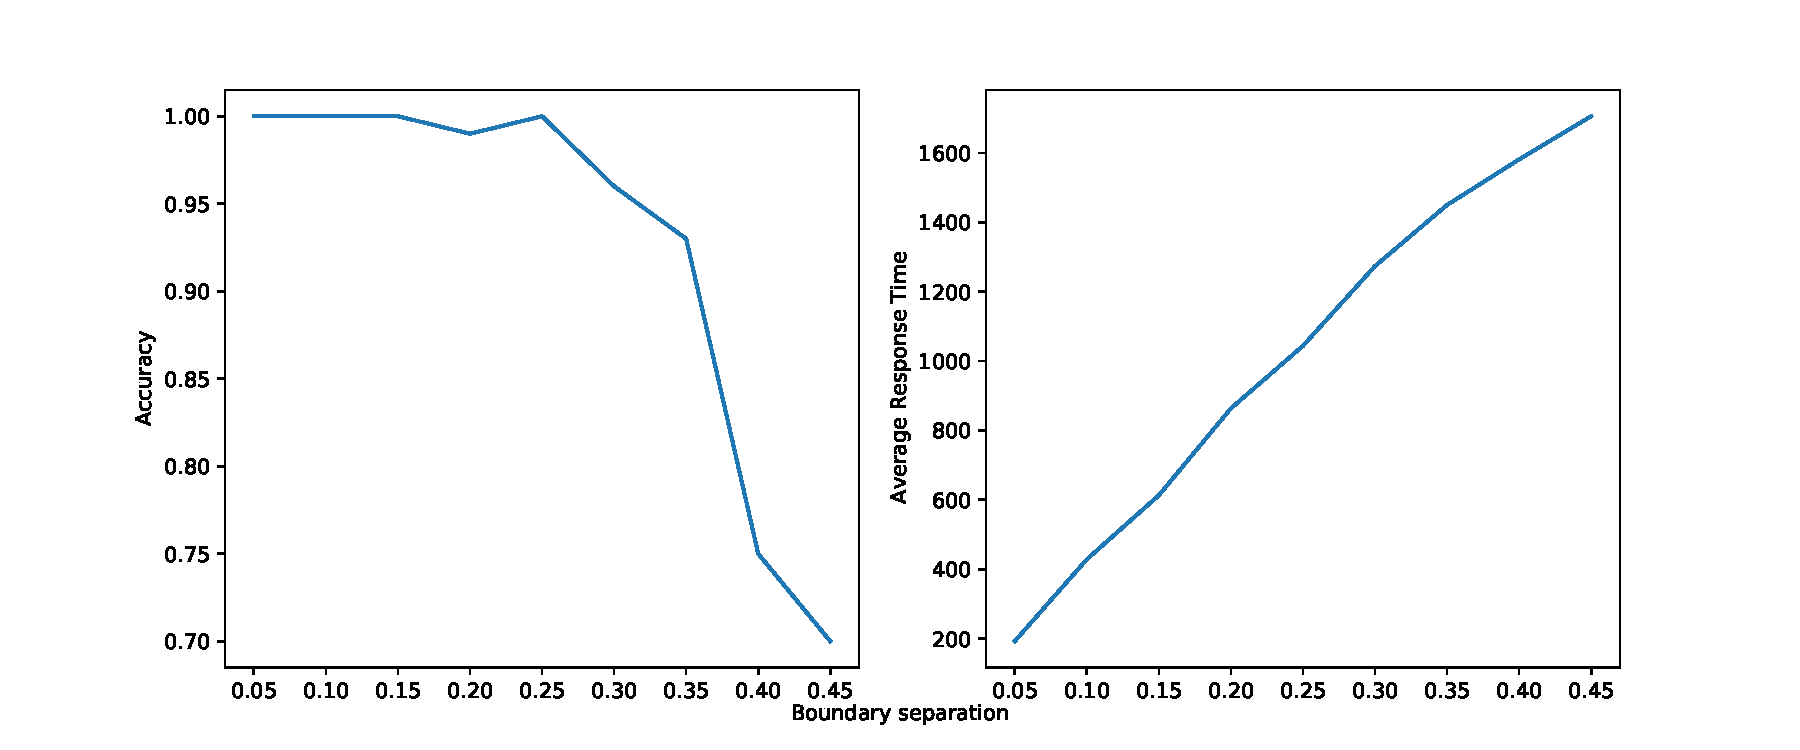
\includegraphics[width=0.8\textwidth]{figures/part1/task2/varying_boundary_separation.pdf}
  \caption{Effect of varying drift rate mean and boundary separation on accuracy and average response times}
  \label{fig:varyingboundaryseparation}
\end{figure}

\subsection{Task (c): Prior information (4)}

To incorperate this prior information, we can simply place the starting point of our simulations closer to the positive hypothesis threshold than the negative, specifically, at 0.75 * boundary condition. This will lower the evidence requirements for accepting this hypothesis whilst increasing the evidence requirements for the negative hypothesis. Figure \ref{fig:examplepathswithpriors} illustrates the changing of the starting point, whilst Table \ref{table:priorresponseconstitution} shows how the response constitution has changed. All other parameters have remained the same as those which produced the results in Table \ref{table:responseconstitution}.

\begin{figure}[H]
  \centering
  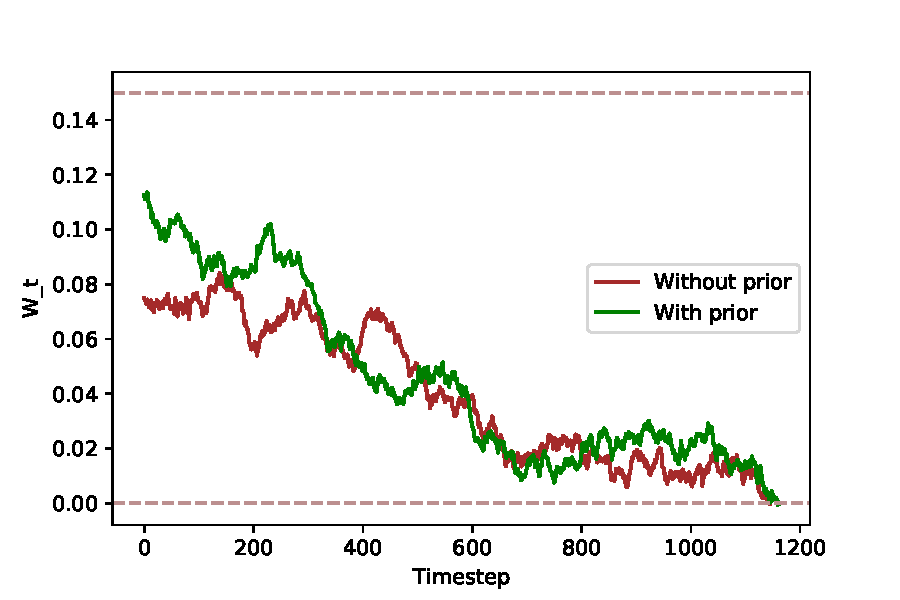
\includegraphics[width=0.8\textwidth]{figures/part1/task3/example_paths_with_priors.pdf}
  \label{fig:examplepathswithpriors}
\end{figure}

\begin{table}[h]
  \begin{tabular}{|l|l|l|}
  \hline
  \textbf{Correct}            & \textbf{Incorrect}          & \textbf{Timeout}            \\ \hline
  \multicolumn{1}{|c|}{1.36\%} & \multicolumn{1}{c|}{34.2\%} & \multicolumn{1}{c|}{52.2\%} \\ \hline
  \end{tabular}
  \centering
  \caption{Response constitution with priors incorperated (1000 trials)}
  \label{table:priorresponseconstitution}
\end{table}

\subsection{Task (d): Group differences (5)}

FILL OUT THIS ANSWER ASAP.

\section{Part 2: Model fitting (77 points)}

\subsection{Task (a): Exploring the data (4)}

Table \ref{table:participantcounts} shows how many rewards each participant received during the trials, and the number of times each participant chose stimulus B over the trials.

If a participant were to choose randomly between the two stimuli in each trial, the expected number of rewards received would be 132. All participants performed better than this random expectation, and so we can deduce that learning took place to some extent during the trials. On the other hand, the top performing participant received 165 rewards during the trials, revealing that the range of rewards received is small over participants.

\subsection{Task (b): Simulations (7)}

\begin{figure}[H]
  \centering
  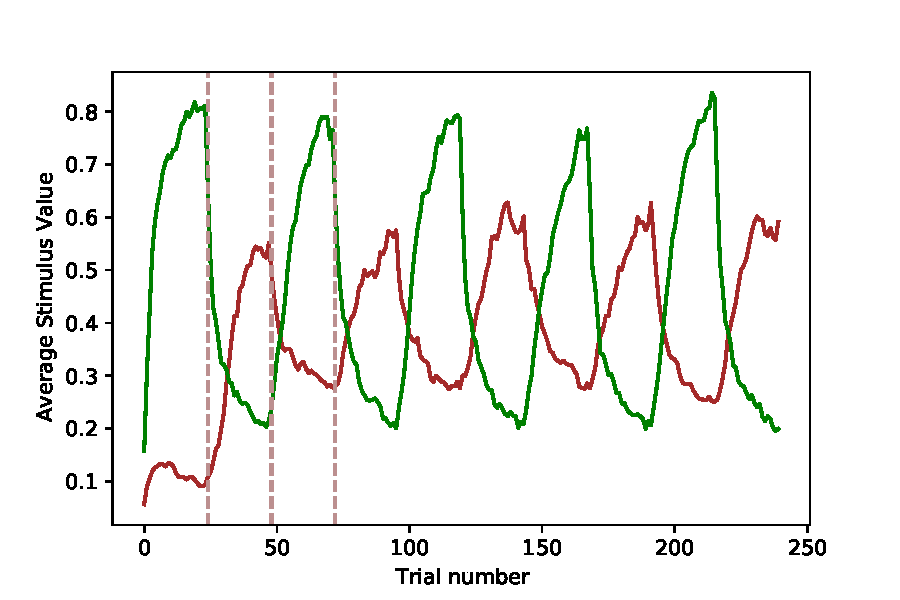
\includegraphics[width=0.4\textwidth]{figures/part2/task2/average_stimulus_values.pdf}
  \caption{Average stimulus values over over 100 simulations}
  \label{fig:averagestimulusvalues}
  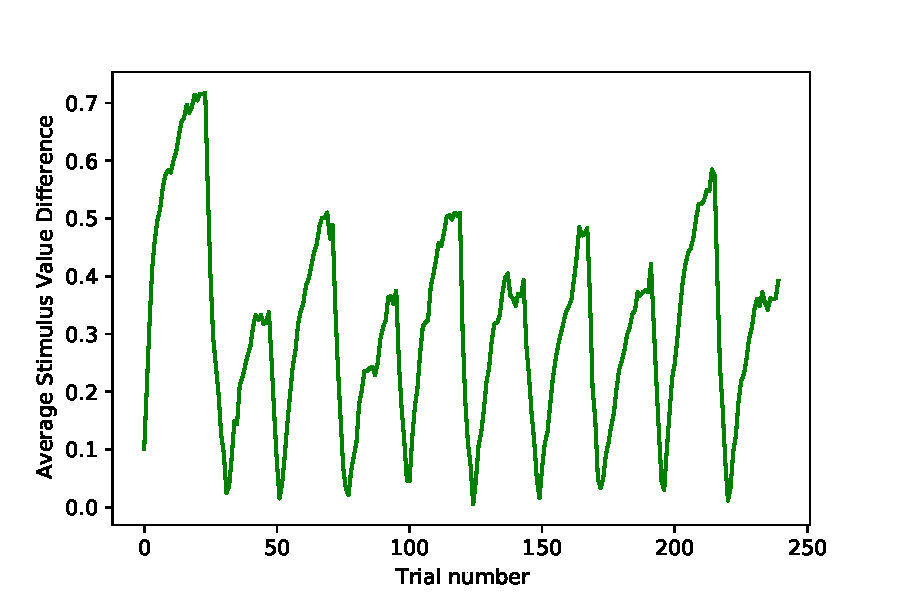
\includegraphics[width=0.4\textwidth]{figures/part2/task2/average_stimulus_value_difference.pdf}
  \caption{Average stimulus value difference over over 100 simulations}
  \label{fig:averagestimulusvaluedifference}
\end{figure}

Figure \ref{fig:averagestimulusvalues} shows the stimulus values for for 240 trials, averaged over 100 simulations. It can be seen that the values tend towards the value of the underlying probability of reward. Vertical lines at trial 24 and 48 show the times at which the underlying reward distribution changed. This evolution makes sense as the reinforcement model begins to build a good reward likelihood for each stimulus, which changes every 24 trials, causing the model to have to approximate different probabilities.

Figure \ref{fig:averagestimulusvaluedifference} shows the difference between the values of the stimulus throughout the trials. This can be interpreted as how likely the model is to choose one stimulus over the other. On the approach to a reward distribution change, the difference between values becomes larger, indicating more certainty of one stimulus over the other. Once the reward distribution changes, the difference between stimulus value diminishes to near 0.

\subsection{Task (c): Exploring parameter settings (6)}

\begin{figure}[H]
  \hspace*{-5cm}
  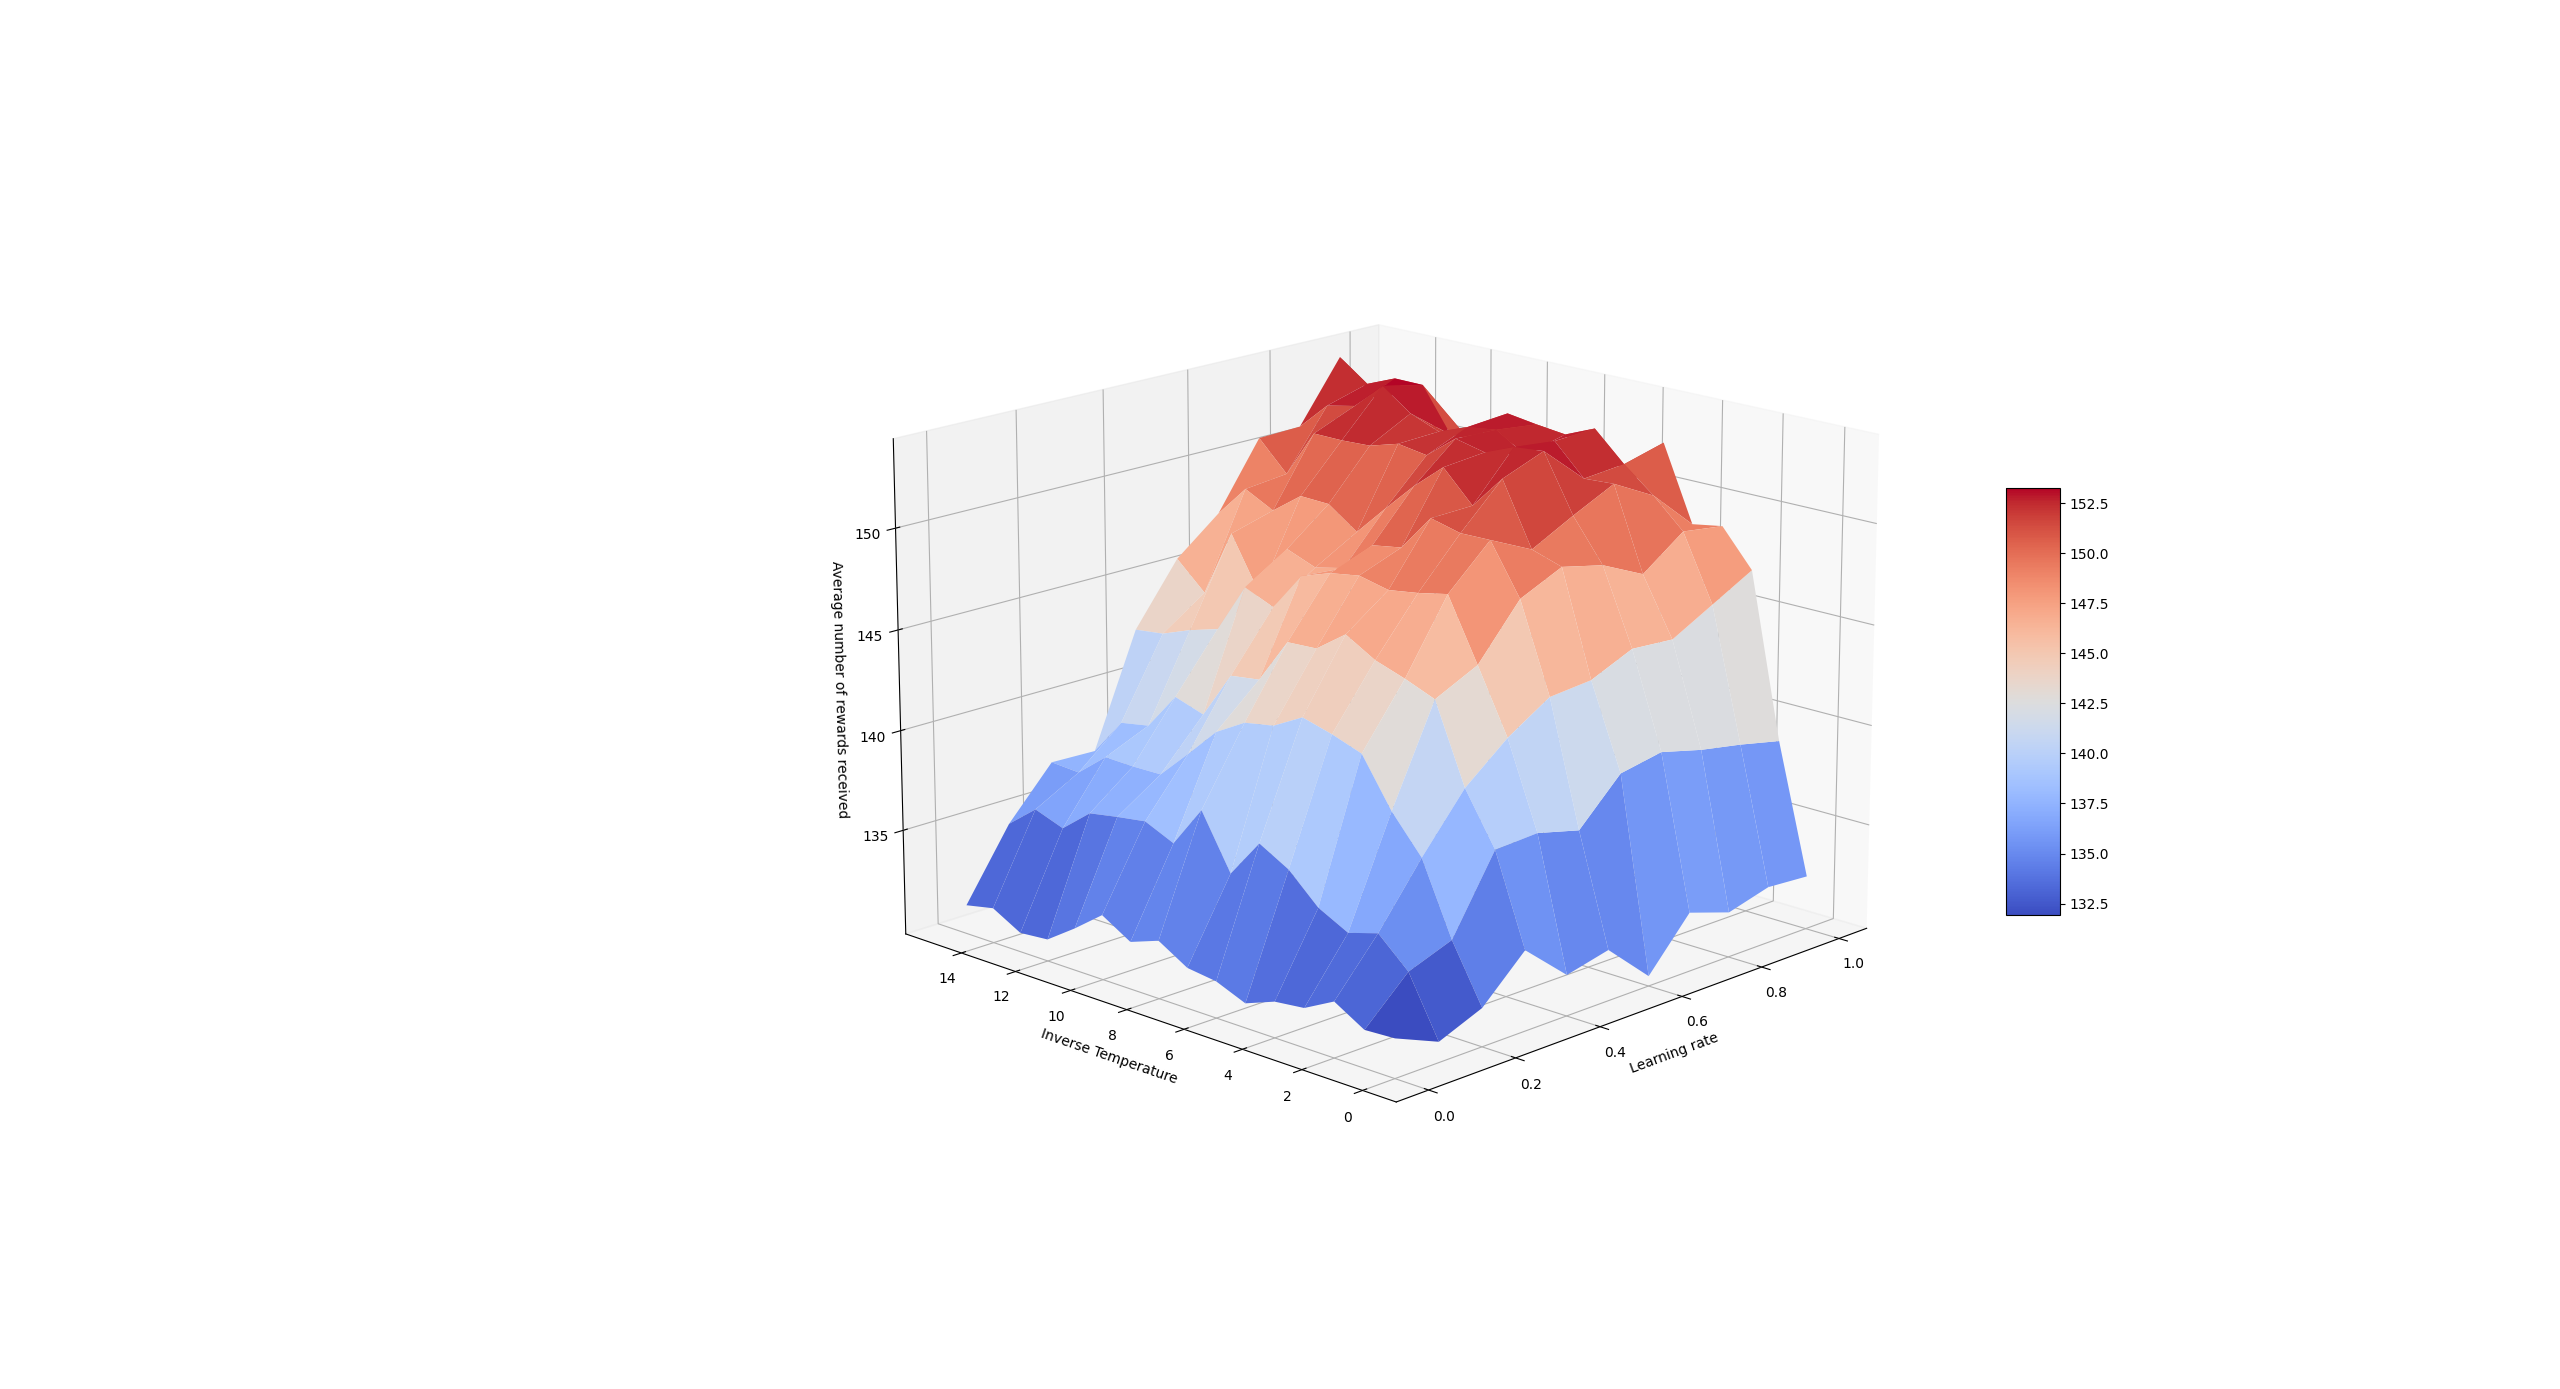
\includegraphics[width=1.4\textwidth]{figures/part2/task2/varying_parameters.png}
  \caption{Effect of varying Learning Rate and Inverse Temperature on Average Rewards Received}
  \label{fig:varyingparameters}
\end{figure}

Figure \ref{fig:varyingparameters} shows the effect of varying the model parameters on the number of rewards received over all trials. The graph is colour coded by the z axis, average number of rewards received, to allow for a better interpretation. It shows that the learning rate effects the rewards received greatly. As the learning rate increases from 0, the average number of rewards increases with it, until it begins to plateau at around 0.6. The same goes for inverse temperature. As inverse temperature increases from 0 to 5, the average number of rewards received increases rapidly, then begins to plateau.

\subsection{Task (d): Likelihood function (6)}

The negative log likelihood for the second participant is 96.256. Listing \ref{listing:part2functionality} contains the function used to calculate this.

\subsection{Task (e): Model fitting (7)}

The following parameter optimizations were performed using the Nelder-Mead method.

\begin{table}[H]
  \centering
  \begin{tabular}{@{}lll@{}}
  \toprule
                      & Mean    & Variance     \\ \midrule
  Learning Rate       & 0.369 &  0.0154  \\
  Inverse Temperature & 5.683 &  1.647    \\ \bottomrule
  \end{tabular}
  \caption{Mean and variance of fitted parameters over all participants}
  \label{table:paramaterstatistics}
\end{table}

\begin{figure}[H]
  \centering
  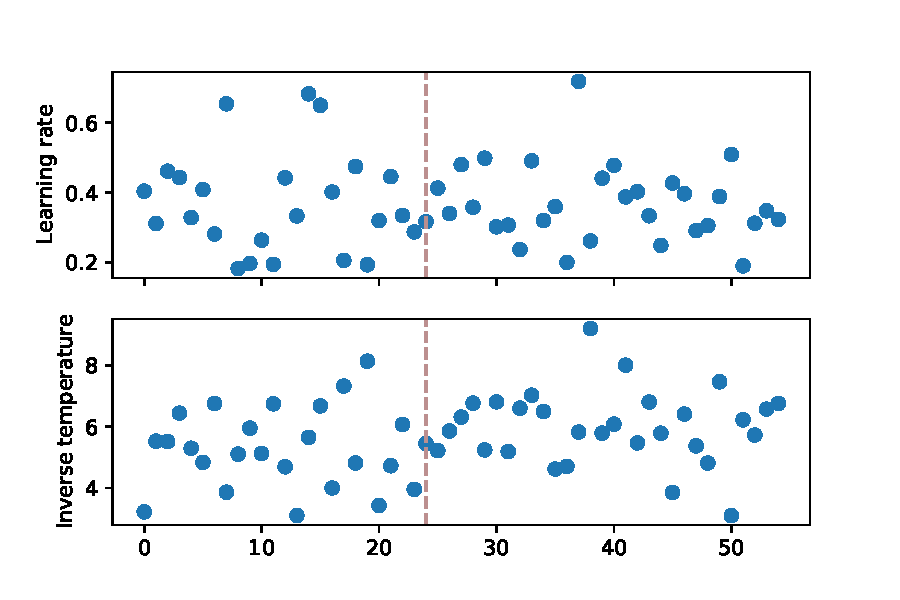
\includegraphics[width=0.8\textwidth]{figures/part2/task5/individual_optimized_parameters.pdf}
  \caption{Optimized parameter fits for individual participants}
  \label{fig:individualoptimizedparameters}
\end{figure}

When using Nelder-Mead, all the parameter values found in figure \ref{fig:individualoptimizedparameters} are within a sane range, even with a non constrained optimization. This is not the case for BFGS optimization, which tended to produce large and unreasonable values. As such, this justified the switch from the recommended optimization strategy.

The dotted line in figure \ref{fig:individualoptimizedparameters} shows the divide between the 24 MDD patients and the 31 healthy control participants. On visual inspection there does not seem to be a difference between these types of participant's optimal parameters.

Pearson's correlation coefficient between estimated parameters among all participants shows no particular significance, a value of -0.209 between the learning rate and inverse temperature. Further, the group specific correlations do not yield anything of significance, with Pearson correlation coefficients of -0.250 and -0.172 for the MDD and healthy participants respectively.


\subsection{Task (f): Group Comparison (5)}

As the assumption of equal variance cannot be assumed, Welch's t-test is suitable for ascertaining whether the MDD and control groups have significantly different estimated parameter distributions for the reinforcement model. For these samples, we have 53 degrees of freedom. Table \ref{table:ttest} shows the results from said test. We can interpret these results by setting a value for what we can consider 'significant'. In this case 0.05 will be used. We observe that the p-value for the learning rate is above this, in which case we can accept the hypothesis that the two groups have similar distributions. In the case of inverse temperature, we observe a value of 0.049, which suggests that we should reject the hypothesis that the two groups have similar distributions. 


\begin{table}[H]
\begin{tabular}{@{}lll@{}}
  \toprule
              & t-statistic & p-value \\ \midrule
Learning Rate & 0.100       & 0.921   \\
Inverse Temp. & -2.020      & 0.049   \\ \bottomrule
\end{tabular}
\caption{Welch's t-test between the two groups of participants (MDD and control)}
\label{table:ttest}
\end{table}


% References
\printbibliography

% Appendices
\begin{appendices}
  
  \begin{table}
    \begin{tabular}{ccc}
      \toprule
      Participant &    Rewards Received &    Times chosen Stimulus B \\
      \midrule
      0  &  154 &   95 \\
      1  &  139 &  106 \\
      2  &  143 &  100 \\
      3  &  156 &  100 \\
      4  &  156 &   96 \\
      5  &  145 &  109 \\
      6  &  134 &  119 \\
      7  &  165 &   98 \\
      8  &  137 &   85 \\
      9  &  151 &   95 \\
      10 &  140 &   96 \\
      11 &  144 &   92 \\
      12 &  144 &  126 \\
      13 &  151 &  106 \\
      14 &  143 &  102 \\
      15 &  158 &   96 \\
      16 &  146 &   78 \\
      17 &  139 &  122 \\
      18 &  161 &  104 \\
      19 &  155 &   43 \\
      20 &  149 &  111 \\
      21 &  145 &   95 \\
      22 &  157 &   89 \\
      23 &  154 &   80 \\
      24 &  156 &  125 \\
      25 &  146 &   88 \\
      26 &  147 &  131 \\
      27 &  141 &   93 \\
      28 &  145 &   82 \\
      29 &  149 &   97 \\
      30 &  152 &   73 \\
      31 &  153 &  102 \\
      32 &  150 &   92 \\
      33 &  149 &   98 \\
      34 &  144 &  123 \\
      35 &  156 &  112 \\
      36 &  163 &  110 \\
      37 &  151 &  108 \\
      38 &  157 &  106 \\
      39 &  159 &   90 \\
      40 &  160 &   92 \\
      41 &  155 &   86 \\
      42 &  146 &   82 \\
      43 &  152 &   87 \\
      44 &  155 &   82 \\
      45 &  155 &   92 \\
      46 &  148 &  100 \\
      47 &  145 &   59 \\
      48 &  150 &   76 \\
      49 &  151 &   97 \\
      50 &  142 &   88 \\
      51 &  150 &  112 \\
      52 &  163 &   61 \\
      53 &  149 &  101 \\
      54 &  148 &   78 \\
      \bottomrule
    \end{tabular}
    \caption{Rewards received and number of times stimulus B was chosen over all trials for each participant}
    \label{table:participantcounts}
  \end{table}

% MATLAB Functions
\section{Python Code}

\begin{listing}
  \inputminted{python}{../part1helpers.py}
  \caption{Part 1 main functionality}
  \label{listing:part1functionality}
\end{listing}

\begin{listing}
  \inputminted{python}{../part2/part2helpers.py}
  \caption{Part 2 main functionality}
  \label{listing:part2functionality}
\end{listing}

\end{appendices}

\end{document}

